\begin{figure}
    \begin{subfigure}{0.47\textwidth}
        \centering
        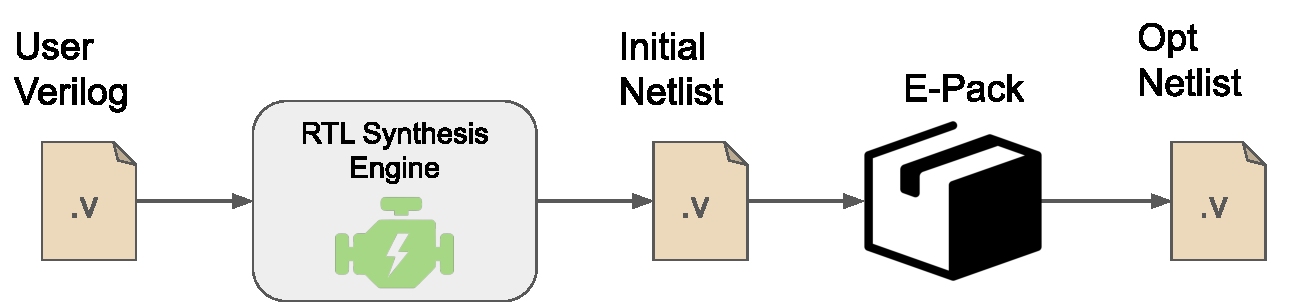
\includegraphics[width=\textwidth]{img/flow.pdf}
        \caption{The design flow integrating \shortname{} with existing RTL tools.}\label{fig:flow:rtl}
    \end{subfigure}
    \hfill\vspace{4mm}
    \begin{subfigure}{0.47\textwidth}
        \centering
        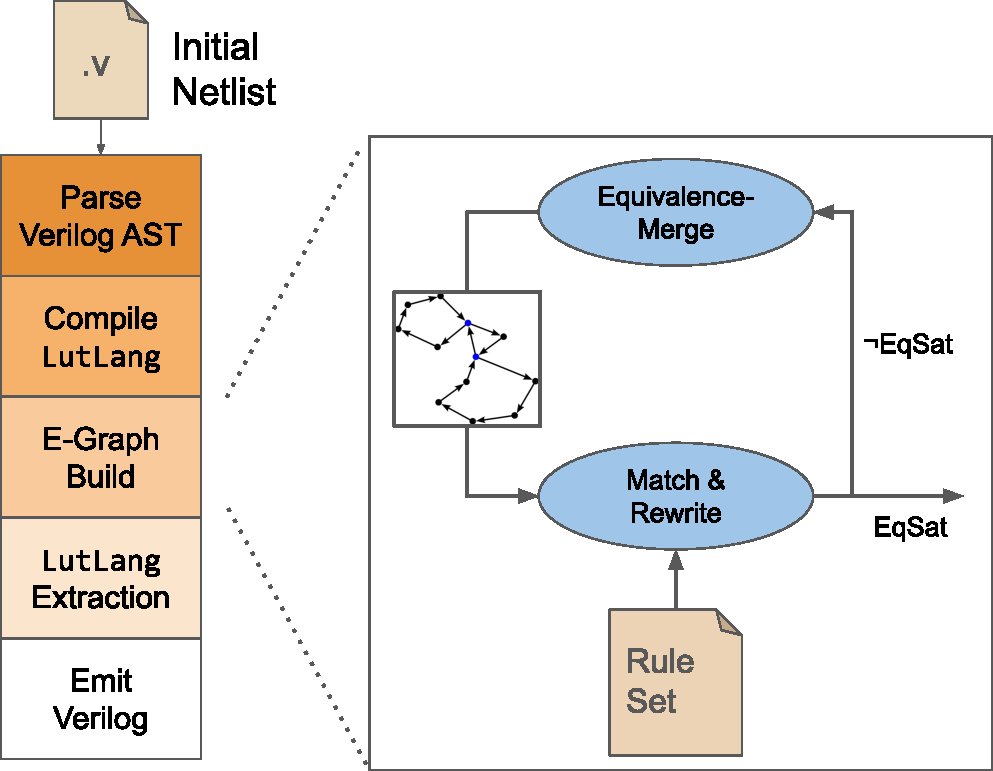
\includegraphics[width=\textwidth]{img/egraph.pdf}
        \caption{The compilation steps internal to \shortname{} Verilog tool.}\label{fig:flow:egraph}
    \end{subfigure}
    \caption{Diagrams of the top-level integration of \shortname{} into existing tool flows and internal compiler architecture.}\label{fig:flow}
\end{figure}

\section{Tool Flow}\label{sec:flow}

While constructing the e-graph is the crux of \shortname{}, there are several
other important components to consider in the full design flow. In order to
test our hypothesis, \shortname{} must be compatible with existing synthesis
flows, and the rewritten circuits must be verified. Fig.~\ref{fig:flow}
provides an overview on both the integration with existing RTL flows and the
internal compiler architecture. The following sections will describe each step
in more detail.

\subsection{Extraction}\label{sec:flow:extraction}
Regardless of whether equality saturation is achieved or not, the quality of
the output circuit still largely depends on the extraction technique used. In
short, \textit{extraction} is the process of selecting the ``best'' circuit
from the e-graph. Given that a saturated e-graph can contain hundreds of
thousands of e-nodes across tens of thousands of e-classes, a greedy extraction
algorithm is the most pragmatic. The greedy extractor iterates over the
e-classes, updating the cost of the cheapest e-node until the database of costs
no longer change. Whenever possible, our compiler uses the built-in
functionality of the egg e-graph Rust library~\cite{docsEgg}. However, e-graph
extraction itself is an ongoing research area~\cite{smoothe,
    sparsextract,esynth}, and future work should experiment with more capable
extraction algorithms. Aside from increases in compile time, better extraction
has the potential to raise the QoR yet another level. In any case, the greedy
cost of a LUT is always one plus the sum of the costs of its children nodes.
Further interactions between extraction and the rewrite rule set are further
explained in Section~\ref{sec:results:margin}.

\subsection{Verilog Support}\label{sec:flow:verilog}
In order for our compiler to be compatible with as many existing design flows
as possible, some level of Verilog support is necessary. Our compiler supports
a subset of Verilog 2001~\cite{verilog}, as required to represent structural
netlists. This includes support for non-ANSI C style module declarations,
wires, and module instantiations with named port connections. With Verilog
support, we are able to test \shortname{} with tool flows that use
Yosys~\cite{yosys} or Vivado~\cite{vivado}. On the backend, our compiler also
emits an updated Verilog netlist.

\subsection{Verification}\label{sec:flow:verification}
While formal verification is not the primary focus of this work, using e-graphs
as a formal reasoning tool helps to build trust in our synthesis results. In
fact, e-graphs were originally designed for automated theorem
proving~\cite{eggpaper}. Thus, constructing proofs that demonstrate equivalence
between the original and remapped netlist is a built-in feature of
\shortname{}. However, we also use two other independent sources of
verification. For combinational netlists, our middle end can do exhaustive
functional testing. Lastly, we use Yosys~\cite{yosys} for its SAT-driven
equivalence checking capabilities. All in all, the mixed usage of these
verification techniques build confidence in the robustness of our technology
mapper built around e-graphs.